
%(BEGIN_QUESTION)
% Copyright 2010, Tony R. Kuphaldt, released under the Creative Commons Attribution License (v 1.0)
% This means you may do almost anything with this work of mine, so long as you give me proper credit

Determine the temperature of the RTD, given $V_{CD}$ = 140.5 millivolts and $V_{EF}$ = 140.1 millivolts:

$$\includegraphics[width=15.5cm]{i00631x01.eps}$$

Assume a 1 k$\Omega$ RTD with $\alpha = 0.00385$, and all wire resistances completely unknown (not assumed to be equal).

\underbar{file i00631}
%(END_QUESTION)





%(BEGIN_ANSWER)

$V_{RTD}$ = 140.1 mV 

\vskip 10pt

$R_{RTD}$ = 1167.5 $\Omega$

\vskip 10pt

$T$ = 43.5 $^{o}$C = 110.31 $^{o}$F (both values calculated from formula, not table)

%(END_ANSWER)





%(BEGIN_NOTES)


%INDEX% Measurement, temperature: RTD (4-wire with cable resistance)

%(END_NOTES)

